% !TeX spellcheck = en_US
\documentclass[
english,
openany,
draft = false,
twoside = true,
fleqn
]{scrbook}
\usepackage{learning-notes}

\author{Huu Duc Nguyen}
\authordegreefront{}
\authordegreeback{ M.Sc.}
\subject{Mathematics}
\title{Mathematics Notes}
\date{27 April 2022}

\begin{document}
\setlength{\abovedisplayskip}{3pt}
\setlength{\belowdisplayskip}{3pt}

\frontmatter
\TitlePage
\tableofcontents

\mainmatter
% !TeX spellcheck = en_GB
\chapter*{Abbreviations}
\addcontentsline{toc}{chapter}{Abbreviations}

\begin{acronym}[LONGEST]
\acro{AI}{Artificial Intelligence}
\acro{AGI}{Artificial General Intelligence}
\acro{ML}{Machine Learning}
\acro{DL}{Deep Learning}
\acro{CS}{Computer Science}
\acro{CV}{Computer Vision}
\acro{RL}{Reinforcement Learning}
\acro{NLP}{Natural Language Processing}
\acro{GPU}{Graphics Processing Unit}
\acro{CPU}{Central Processing Unit}

% Conferences
\acro{ICML}{\href{https://icml.cc/}{International Conference on Machine Learning}}

\acro{prob}[prob.]{probability}
\acro{param}[params.]{parameters}
\acro{algor}[algor.]{algorithms}
\acro{info}[info.]{information}
\acro{aka}[a.k.a.]{also known as}
\acro{wrt}[w.r.t.]{with regard to}
\acro{no}[no.]{number of}
\acro{func}[func.]{function}
\acro{vs}[vs.]{versus}
\acro{freq}[freq.]{frequency}
\acro{st}[s.t.]{subject to}

\acro{iid}[i.i.d.]{independent \& identically distributed}
\acro{LSI}{linear shift invariant}
\acro{pdf}[pdf.]{Probability Density Function}
\acro{MLE}{Maximum Likelihood Estimation}
\acro{MAP}{Maximum A Posteriori}
\acro{MoG}{Mixture of Gaussians}
\acro{SVM}{State Vector Machine}

% Gradient descent
\acro{GD}{Gradient Descent}
\acro{SGD}{Stochastic Gradient Descent}
\acro{nag}[NAG]{Nestorov Accelerated Gradient}
\acro{rmsprop}[RMSprop]{Root mean squared prop}
\acro{adam}[Adam]{Adaptive moment estimation}

\acro{SVD}{Singular Value Decomposition}
\acro{PCA}{Principal Component Analysis}
\acro{LDA}{Linear Discriminant Analysis}
\acro{KL}[KL]{Kullback–Leibler}
\acro{IG}{Information Gain}

% Mathematics & Optimization
\acro{KKT}{Karush-Kuhn-Tucker}
\acro{RBF}{Radial basic function}
\acro{iff}[i.f.f.]{if and only if}
\acro{LP}{Linear Programming}
\acro{QP}{Quadratic Programming}
\acro{LQR}{Linear Quadratic Regulator}
\acro{iLQR}{Iterative Linear Quadratic Regulator}
\acro{MPC}{Model Predictive Control}
\acro{FLM}{Fitted Local Model}
\acro{FFT}{Fast Fourier Transform}

% Neural-network-related term
\acro{MLP}{Multi-Layer Perceptron}
\acro{relu}[ReLU]{Rectified Linear Unit}
\acro{BPTT}{Backpropagation through time}
\acro{RNN}{Recurrent Neural Network}
\acro{LSTM}{Long short-term memory}
\acro{CNN}{Convolutional Neural Network}
\acro{GNN}{Graph Neural Network}
\acro{CONV}{Convolutional}
\acro{FC}{Fully Connected}
\acro{VAE}{Variational Auto-Encoders}
\acro{GAN}{Generative Adversarial Network}
\acro{DCGAN}{Deep Convolutional Generative Adversarial Network}
\acro{CGAN}{Conditional Generative Adversarial Network}
\acro{SRGAN}{Super Resolution Generative Adversarial Network}
\acro{ESRGAN}{Enhanced Super Resolution Generative Adversarial Network}
\acro{ResNet}{Residual Network}
\acro{BatchNorm}{Batch Normalization}
\acro{IN}{Instance Normalization}
\acro{AdaIN}{Adaptive Instance Normalization}
\acro{NAS}{Neural Architecture Search}

% Robotics
\acro{dof}[DOF]{degrees of freedom}
\acro{ee}[EE]{end-effector}
\acro{DH}[D-H]{Denavit–Hartenberg}

% Probabilistic Robotics
\acro{KF}{Kalman Filter}
\acro{EKF}{Extended Kalman Filter}
\acro{IF}{Information Filter}
\acro{EIF}{Extended Information Filter}
\acro{MHEKF}{Multi-Hypothesis Extended Kalman Filter}

% Reinforcement learning related
\acro{HMM}{Hidden Markov Model}
\acro{MDP}{Markov Decision Process}
\acro{POMDP}{Partially Observable Markov Decision Process}
\acro{TSP}{Travelling Salesman Problem}
\acro{A3C}{Asynchronous advantage actor-critic}
\acro{SAC}{Soft actor-critic}
\acro{DQN}{Deep Q-learning}
\acro{DDP}{Differential Dynamic Programming}
\acro{dagger}[DAgger]{Dataset Aggregation}
\acro{CEM}{Cross-entropy Method}
\acro{MCTS}{Monte-Carlo Tree Search}
\acro{MBA}{Model-based Acceleration}
\acro{MVE}{Model-based Value Expansion}
\acro{MBPO}{Model-based Policy Optimization}
\acro{UCB}{Upper Confidence Bounce}
\acro{PAC}{Probably Approximately Correct}
\acro{CQL}{Conservative Q-learning}
\acro{MOPO}{Model-Based Offline Policy Optimization}
\acro{IRL}{Inverse Reinforcement Learning}
\acro{MaxEnt}{Maximum Entropy}
\acro{MAML}{Model-Agnostic Meta-Learning}
\acro{OPE}{Off-policy evaluation}
\acro{LSTD}{Least-squares temporal difference}
\acro{LSPI}{Least-squares policy iteration}

% Computer vision related
\acro{DPM}{Deformable Part Model}
\acro{HOG}{Histogram of Oriented Gradients}
\acro{SSIM}{Structural Similarity Index}
\acro{SRCNN}{Super Resolution Convolutional Neural Network}
\acro{PPL}{Perceptual path length}
\acro{FID}{Fréchet inception distance}

% Psychology related
\acro{US}{unconditioned stimuli}
\acro{UR}{unconditioned response}
\acro{CS}{conditioned stimuli}
\acro{CR}{conditioned response}
% Neuroscience related
\acro{CNS}{central nervous system}
\acro{PNS}{peripheral nervous system}
\acro{EEG}{Electroencephalography}
\acro{fMRI}{Functional Magnetic Resonance Imaging}
\acro{ECoG}{Electrocorticography}
\acro{LFP}{Local Field Potentials}
\acro{BCI}{Brain-Computer Interface}
\acro{BMI}{Brain Machine Interface}
\acro{NMP}{neuromotor prostheses}
\acro{PSD}{Power Spectral Density}

\end{acronym}

% !TeX spellcheck = en_US
\chapter{Introduction}

\section{Resources}
\begin{itemize}
	\item \href{https://youtube.com/playlist?list=PLZHQObOWTQDPD3MizzM2xVFitgF8hE_ab}{Essence of linear algebra | 3Blue1Brown}
	\item \href{https://youtube.com/playlist?list=PLZHQObOWTQDMsr9K-rj53DwVRMYO3t5Yr}{Essence of calculus | 3Blue1Brown}
	\item \href{https://youtube.com/playlist?list=PLE7DDD91010BC51F8}{Linear Algebra | MIT 18.06 Spring 2005}
\end{itemize}
\chapter{Matrix}

\section{Singular Value Decomposition}

\ac{SVD}

\href{https://machinelearningcoban.com/2017/06/07/svd/}{MLcoban.com}
% !TeX spellcheck = en_US
\chapter{Probabilities}
\label{cha:probabilities}
For more examples, exercises with solutions, check:
\begin{itemize}
	\item \citeaustitle{bishop2006pattern}
\end{itemize}

\section{General}
\subsection{Basic Definitions}
\begin{itemize}
	\item If $x$ is discrete: $\underset{x}{\sum} p(x) = 1$ with $\forall$ $0 \leq p(x) \leq 1$
	\item If $x$ is continuous: $\displaystyle \int p(x) \,dx = 1 \Rightarrow \exists$ a \textbf{\ac{pdf}}\\
	$p(x)$ can take any positive value, as long as \(\displaystyle \int p(x) \,dx = 1\) \tab 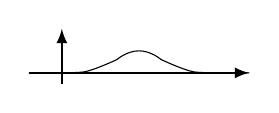
\begin{tikzpicture}[scale=1.4]
		\draw[-latex, thick] (-1,0)--(1,0);
		\draw[-latex, thick] (-.7,-.1)--(-.7,.4);		
		\draw plot [smooth, tension=1] coordinates {(-.2,.121) (0,.2) (.2,.121)};
		\draw plot [smooth, tension=.4] coordinates {(-1,0) (-.5,.00876) (-.2,.121)};
		\draw plot [smooth, tension=.4] coordinates {(.2,.121) (.5,.00876) (1,0)};
	\end{tikzpicture}	
	\note: theoretically $p(x) = 0, \forall x$
	\item Common types
	\begin{align*}
		& \text{Joint probability:} 		&& p(x_i, y_i) 	&& = p(X=x_i, Y=y_i) \\
		& \text{Marginal probability:} 		&& p(x_i) 		&& = p(X=x_i) \\
		& \text{Conditional probability:} 	&& p(y_i | x_i) && = p(Y=y_i|X=x_i)
	\end{align*}	
	\item Sum rule: $\displaystyle \sum$ joint \ac{prob} = marginal \ac{prob}\\
	$\Rightarrow$ Marginalization	
	\begin{itemize}
		\item discrete variable: $\displaystyle p(x)=\underset{y}{\sum} p(x, y)$
		\item continuous variable: $\displaystyle p(x) = \int p(x,y) dy$
	\end{itemize}
	\item Product rule: Product of marginal \ac{prob} and conditional \ac{prob} = joint \ac{prob}
\end{itemize}

\subsection{Expectation}
\label{subsec:expectation}
\begin{align*}
	& \text{For variable $x$:} && \expectation{x} = \underset{x}{\sum}x.p(x) && = \int p(x)x\text\ {d}x \\
	& \text{For function $f(\cdot)$:} && \expectation{f(x)} = \underset{x}{\sum}f(x).p(x) && = \int p(x)f(x)\ \text{d}x
\end{align*}

\subsection{Independence and Variability}
\begin{itemize}
	\item Independence. \Eg: $x, y$ are independent, then
	\[\begin{cases}
		p(x|y) = p(x)\\
		p(y|x) = p(y)
	\end{cases}
	\Leftrightarrow p(x,y) = p(x).p(y)\]	
	\item Variability
	\begin{itemize}
		\item variance: how much variability there is in $f(x)$ around its mean value $\expectation{f(x)}$\\
		$var [f] = \expectation{\left(f(x)-\expectation{f(x)}\right)^2} = \expectation{f(x)^2} - \expectation{f(x)}^2$
		\item covariance: for two random variables $x, y$\\
		$cov [x, y] = \mathbb{E}_{x,y}\left[xy\right] - \expectation{x}.\expectation{y}$
		\item covariance matrix: if $x, y$ are vectors
		\begin{align*}
			cov [\textbf{x}, \textbf{y}] &= \mathbb{E}_{\textbf{x},\textbf{y}} \left[ \left\{\textbf{x}-\expectation{\textbf{x}}\right\} \left\{\textbf{y}^T -  \expectation{\textbf{y}^T} \right\} \right]\\
			&= \mathbb{E}_{\textbf{x,y}}\left[\textbf{xy}^T\right] - \expectation{\textbf{x}}.\expectation{\textbf{y}^T}
		\end{align*}
	\end{itemize}
\end{itemize}

\subsection{Bayes Rule}
\label{subsec:bayes-rule}
\begin{align*}
	& p(x_i|y_i).p(y_i) = p(y_i|x_i).p(x_i) = p(x_i, y_i) \\
	\Rightarrow\; &p(y_i|x_i) = \frac{p(x_i|y_i).p(y_i)}{p(x_i)} = \frac{p(x_i|y_i).p(y_i)}{\underset{y}{\sum} p(x_i|y_i).p(y_i)}
\end{align*}
$\Rightarrow$ the \hlb{Bayes equation}:\tab{\color{red} \boxed{\hlre{posterior = \frac{likelihood \times prior}{normalization~factor}}}}

\section{Types of Probability Distributions}
Reference source: \href{https://machinelearningcoban.com/2017/07/09/prob/}{machinelearningcoban.com}.
\subsection{Bernoulli Distribution}
Bernoulli Distribution is a distribution to describe binary discrete variables. It's the case that the variable can only take value in 2 classes $x \in \{0,1\}$. \Eg, the probability of throwing a coin. The Bernoulli distribution is defined with parameter $\lambda \in[0,1]$:
\begin{equation}
	p(x) = \text{Bern}_x[\lambda] = \begin{cases}
		p(x=1) = \lambda\\
		p(x=0) = 1-\lambda
	\end{cases}
\end{equation}
In short form, the above equation can be combined into one:
\begin{equation}
	p(x) = \lambda^x(1-\lambda)^{(1-x)} \Rightarrow
	\begin{cases}
		p(0) = \lambda^0 (1-\lambda)^1 = 1-\lambda \\
		p(1) = \lambda^1 (1-\lambda)^0 = \lambda \\
	\end{cases}
\end{equation}

\subsection{Categorical Distribution}
\label{subsec:categorical-distribution}
\textit{Categorical Distribution} is the generalization of \textit{Bernoulli Distribution} for $K$ classes of the discrete variable $x \in \{ 1, 2, \dots, K\}$. Accordingly, there will be $K$ parameters to describe this \ac{pdf}: $\lambda = [\lambda_1, \lambda_2, \dots, \lambda_K]$, with $\lambda_k \geq 0$ and $\sum \lambda_k = 1$. Each $\lambda_k$ represents the probability to take the output $k$: $p(x = k) = \lambda_k$. In short: $p(x) = \text{Cat}_x [\lambda]$.

Another common way to represent the output is the one-hot vector, $\mathbf{x} \in \{\mathbf{e}_1, \mathbf{e}_2, \dots, \mathbf{e}_K\}$ with $\mathbf{e}_k$ is the $k$-unit vector, which has all 0-element, except the $k$-element equal to 1. \Eg, given 3 classes: $\textbf{e}_1 = [1, 0, 0]^T, \textbf{e}_2 = [0, 1, 0]^T, \textbf{e}_3 = [0, 0, 1]^T$. We will then have:
\begin{equation}
	p(\mathbf{x} = \mathbf{e}_k) = \prod_{j=1}^K \lambda_j^{x_j} = \lambda_k
\end{equation}
because for $\textbf{x}=\textbf{e}_k$, only $x_k=1$, while $x_j = 0, \forall j\neq k$.

\subsection{Univariate Normal Distribution}
Univariate Normal Distribution is also known as the Gaussian distribution. For single dimension data (in 1D): $x \in (-\infty, \infty)$, the mean $\mu \in \mathbb{R}$, and the variance $\sigma^2$ with $\sigma \in \mathbb{R}$.
\begin{equation}
	p(x) = \text{Norm}_x\left[\mu, \sigma^2\right] = \mathcal{N}(\mu, \sigma^2) = \frac{1}{\sqrt{2\pi\sigma^2}}.\text{exp}\left(-\frac{(x-\mu)^2}{2\sigma^2}\right)
\end{equation}
\note
\begin{itemize}
	\item \hlr{Marginals \ac{prob} of Gaussian are again Gaussian.}
	\item When estimating the \ac{param} of a Gaussian, beware the underestimation problem.
	\begin{align*}
		\expectation{\mu_{ML}} &= \mu \\
		\expectation{\sigma^2_{ML}} &= \left(\frac{N-1}{N}\right)\sigma^2 \\
		\Rightarrow \overset{\sim}{\sigma}^2 &= \left(\frac{N}{N-1}\right)\sigma^2_{ML} = \frac{1}{N-1} \sum_{n=1}^{N} (x_n-\hat{\mu})^2
	\end{align*}
\end{itemize}
\begin{figure}[hbt!]
	\centering
	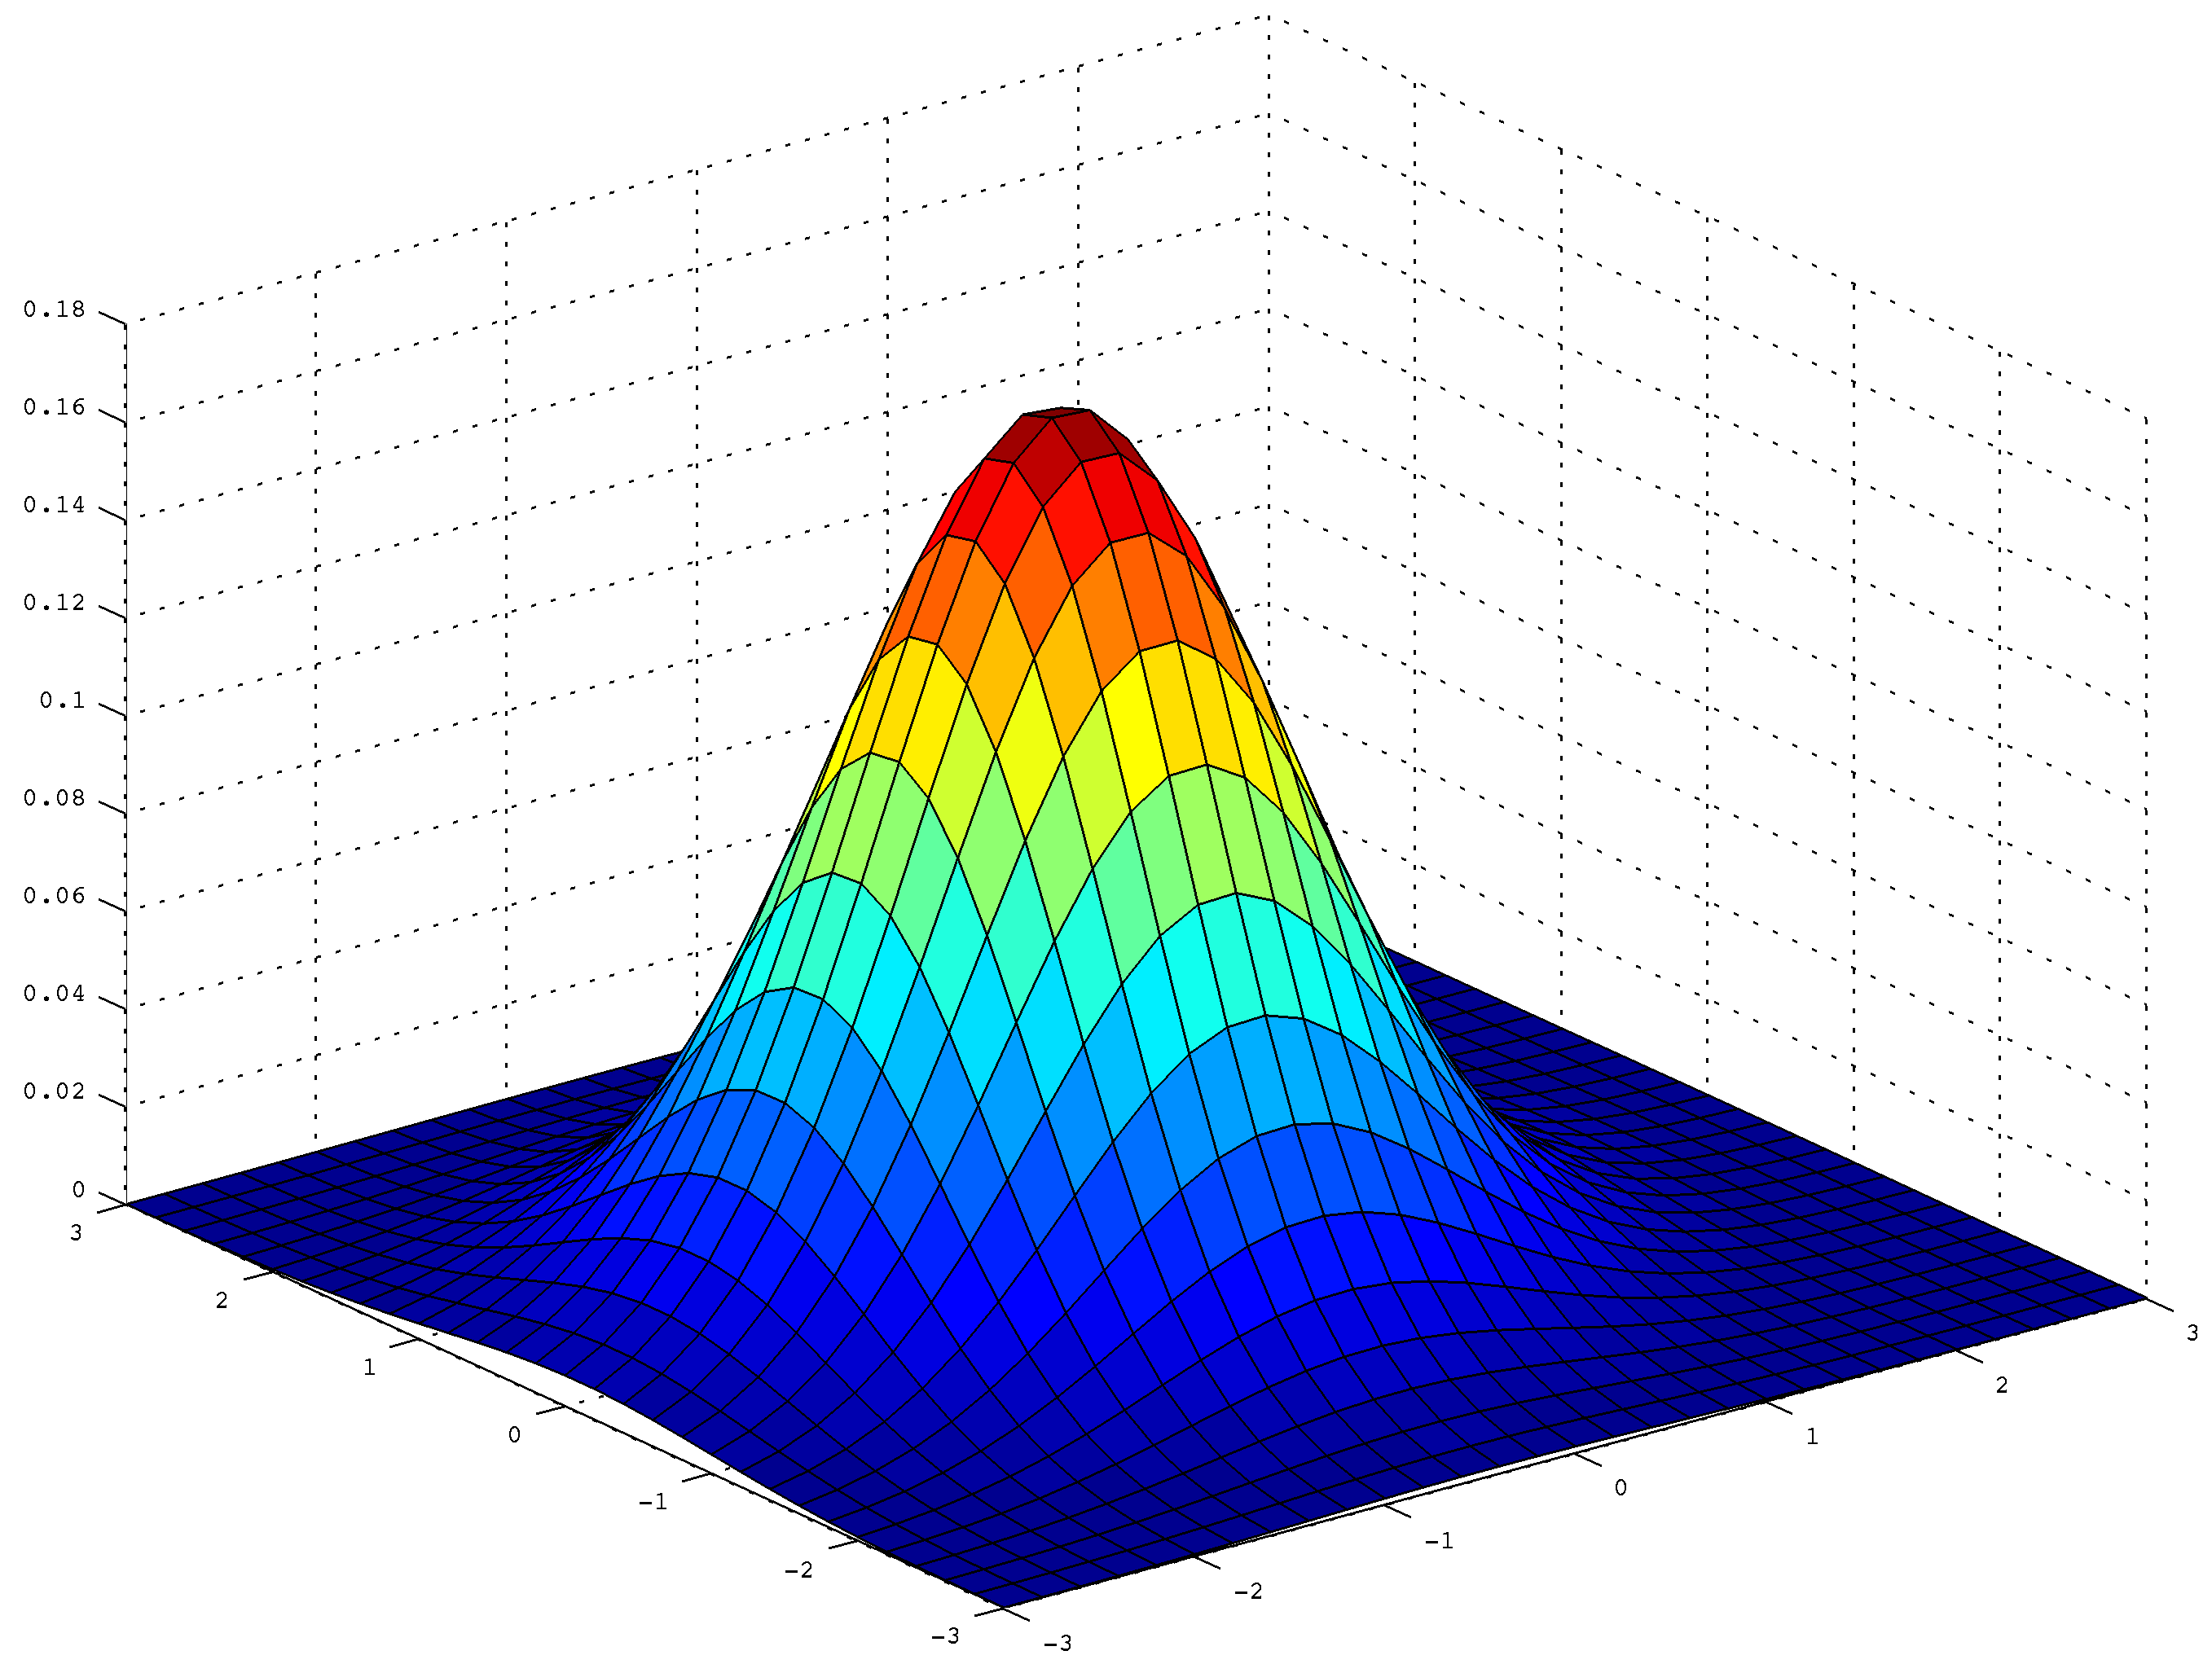
\includegraphics[width=0.7\textwidth]{gaussian-pdf.png}
	\caption{Bivariate Gaussian distribution (\href{https://stats.stackexchange.com/questions/102632/plot-two-dimensional-gaussian-density-function-in-matlab}{src}).}
	\label{fig:relation-ai-ml-dl}
\end{figure}

\subsection{Multivariate Normal Distribution}
\textit{Multivariate Normal Distribution} is the extension of \textit{Univariate Normal Distribution} to multi-dimensional data: $\textbf{x}, \boldsymbol{\mu} \in \mathbb{R}^D, \sigma^2 \Rightarrow \Sigma \in \mathbb{S}^D_{++}$ ($\mathbb{S}^D_{++}$ is the set of positive definite symmetric matrix)
\begin{equation}
	p(x) = \text{Norm}_x [\boldsymbol{\mu}, \Sigma] = \mathcal{N}(\boldsymbol{\mu}, \Sigma) = \frac{1}{2\pi^{D/2}| \Sigma|^{\frac{1}{2}}} . \text{exp} \left( -\frac{1}{2} {(\textbf{x} - \boldsymbol{\mu})^T \Sigma^{-1} (\textbf{x} - \boldsymbol{\mu})} \right)
\end{equation}

\subsection{Beta Distribution}
This distribution describes the parameter for another distributions. \Eg, Dirichlet \ac{pdf} describes Categorical Distribution (\subsecref{subsec:categorical-distribution})
% !TeX spellcheck = en_US
\chapter{Information Theory}
\label{cha:information-theory}
\todo{intro}

\section{Entropy}
\begin{align}
	&p(\textbf{x}) &&-\text{distribution (\eg over observation $\textbf{x}$)}\\
	\mathcal{H}(p) =& -\mathbb{E}_{\textbf{x}\sim p(\textbf{x})} [\log p(\textbf{x})] &&-\text{entropy - how "broad" $p(\textbf{x})$ is}\\
	=& - \sum_{i=1}^{N} p(\textbf{x}_i) \log p(\textbf{x}_i)
\end{align}

Intuition:
\begin{itemize}
	\item How \textit{random} is the variable?\\
	The more random the variable, the higher the entropy (\figref{fig:entropy})
	\item How large is the log \ac{prob} in expectation \textit{under} itself?
	\begin{itemize}
		\item If you mostly see low $\log$ \ac{prob}, then there are many places with similar \ac{prob}, and the entropy, as negative $\log$, would be high (\figref{fig:entropy-high}).
		\item If you mostly see high $\log$ \ac{prob}, then the variable focuses around only a few place, thus, the entropy, as negative $\log$, would be low (\figref{fig:entropy-low}).
	\end{itemize}	
\end{itemize}

\begin{figure}[hbt!]
	\centering
	\begin{subfigure}[b]{0.45\textwidth}
		\centering
		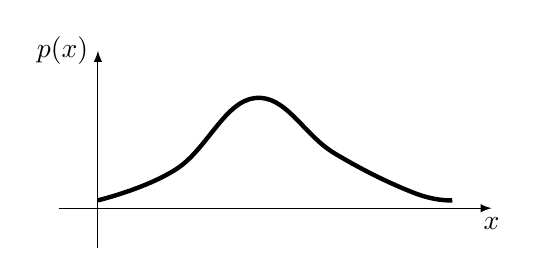
\begin{tikzpicture}
			\draw[-latex] (-.5,0) -- (5,0) node[below] {$x$};
			\draw[-latex] (0,-.5) -- (0,2) node[left] {$p(x)$};
			\draw[ultra thick] plot [smooth, tension=.7] coordinates {(0, 0.1) (1,0.5) (2,1.4) (3,0.7) (4, .2) (4.5,0.1)};
		\end{tikzpicture}
		\caption{Example of $p(x)$ with high entropy.}
		\label{fig:entropy-high}
	\end{subfigure}
	\hfill
	\begin{subfigure}[b]{0.45\textwidth}
		\centering
		\begin{tikzpicture}
			\draw[-latex] (-.5,0) -- (5,0) node[below] {$x$};
			\draw[-latex] (0,-.5) -- (0,2) node[left] {$p(x)$};
			\draw[ultra thick] plot [smooth, tension=.7] coordinates {(1.7,0.1) (2,1.4) (2.2,0.1)};
		\end{tikzpicture}
		\caption{Example of $p(x)$ with low entropy.}
		\label{fig:entropy-low}
	\end{subfigure}
	\caption{Examples of $p(x)$ with different entropy.}
	\label{fig:entropy}
\end{figure}

\section{Cross Entropy}
\label{sec:cross-entropy}
The cross entropy between two given \ac{prob} distributions $p$ and $q$ is defined as:
\begin{equation}
	H(p, q) = \mathbb{E}_p[-\log q]
\end{equation}
With \textbf{p, q} as discrete variables:
\begin{equation}
	H(\textbf{p, q}) = \sum_{i=1}^{C} p_i \log q_i
\end{equation}

\note $\nexists \log (0) \Rightarrow \text{condition: } \textbf{q} >0$

\section{Kullback - Leiber Divergence}

The \ac{KL}-divergence tells:
\begin{itemize}
	\item How \textit{different} are two distributions?
	\item How small is the expected log \ac{prob} of one distribution under another, \hlr{minus entropy}?
\end{itemize}

Example reference: 	\href{https://www.countbayesie.com/blog/2017/5/9/kullback-leibler-divergence-explained}{countbayesie}

\begin{align}
	H &= - \sum_{i=1}^{N} p(x_i) \log p(x_i)\\
	D_{KL}(p || q) &= \sum_{i=1}^N p(x_i) \left[ \log p(x_i) - \log q(x_i) \right]\\
	&= \sum_{i=1}^N p(x_i) \log \frac{p(x_i)}{q(x_i)}\\
	&= \mathbb{E}_{x \sim p(x)} \left[ \log p(x) - \log q(x) \right]
\end{align}
$\Rightarrow$ How many bits of info we expect to loose\\
$\Rightarrow$ \hlb{A function} that we can \hlb{optimized}

\textbf{\color{red} cross entropy = entropy + KL Divergence}
\begin{equation}
	{\color{red} H(p, q) = H(p) + D_{KL}(p || q)}
\end{equation}

\Eg: KL divergence between two normal distributions $\mathcal{N}(\mu_1, \sigma_1)$ and $\mathcal{N}(\mu_2, \sigma_2)$:
\begin{equation}
	D_{KL}(p, q) = \log \frac{\sigma_2}{\sigma_1} + \frac{\sigma_1^2 + (\mu_1 - \mu_2)^2}{2 \sigma_2^2} - \frac{1}{2}
\end{equation}

\underline{\textbf{PSEUDO CODE:}} with $\mu_2=0, \sigma_2 = 1$
\begin{align}
	\mu, \sigma &= \texttt{encoder}(\hat{x})\\
	\texttt{z} &= \mu + \sigma * \texttt{random\_normal(0, 1)}\\
	\texttt{y} &= \texttt{decoder(z)}\\
	\texttt{recon\_loss} &= \texttt{x.log(y) + (1-x)log(1-y)}\\
	\texttt{KL\_loss} &= \frac{1}{2} [ \mu^2 + \sigma^2 - \texttt{log}(\sigma^2 + 1e^{-8}) -1 ]\\
	\texttt{ELBO} &= \texttt{recon\_loss - KL\_loss}\\
	\texttt{loss} &= \texttt{-ELBO}
\end{align}

\section{Mutual Information}
\begin{align}
	&p(x) &&-\text{distribution (\eg over observation $\textbf{x}$)}\\
	\mathcal{H}(p(\textbf{x})) =& -\mathbb{E}_{\textbf{x}\sim p(\textbf{x})} [\log p(\textbf{x})] &&-\text{entropy - how "broad" $p(\textbf{x})$ is}\\
	\mathcal{I}(\textbf{x};\textbf{y}) =& D_{KL} \big(p(\textbf{x,y}) || p(\textbf{x}) p(\textbf{y})\big) &&-\text{mutual information}\\
	=& \mathbb{E}_{(\textbf{x,y}) \sim p(\textbf{x,y})} \left[ \log \frac{p(\textbf{x,y})}{p(\textbf{x})p(\textbf{y})} \right]\\
	=& \mathcal{H}(p(\textbf{y})) - \mathcal{H}(p(\textbf{y|x})) &&-\text{relates to \ac{IG}}
\end{align}
The last equation implies that we can interpret mutual information $\mathcal{I}(\textbf{x};\textbf{y})$ as \ac{IG}, how much more do we know about \textbf{y} after receiving observation about \textbf{x}.

\Eg:
\begin{itemize}
	\item If \textbf{x} and \textbf{y} are independent of each others, then $p(\textbf{x,y}) = p(\textbf{x}) p(\textbf{y})$, thus $\mathcal{I}(\textbf{x};\textbf{y})=0$
	\item If \textbf{x} and \textbf{y} depends on each others more and more, the different between the joint \ac{prob} $p(\textbf{x,y})$ and the product of marginal \ac{prob} $p(\textbf{x}) p(\textbf{y})$ grows, thus the $\mathcal{I}(\textbf{x};\textbf{y})$ is larger.
\end{itemize}
% !TeX spellcheck = en_US
\chapter{Convexity}

\section{Convex Sets}
\begin{itemize}
	\item Definition 1: line connects 2 points of a convex set lies within the set
	\item Definition 2: $\mathcal{C}$ is a convex set if for $\forall x_1, x_2 \in \mathcal{C}$:
	\[ x_\theta = \theta x_1 + (1-\theta) x_2 \in \mathcal{C}, \quad \forall\; 0 \leq \theta \leq 1\]
	\item Hyperplane is a \hlb{convex set}
	\[ a_1x_1 + a_2x_2 + \dots + a_nx_n = \textbf{a}^T\textbf{x} = b, \quad b, a_i \in \mathbb{R}, \quad i \in \mathbb{N} \]
	\item Half-space is a \hlb{convex set}
	\[ a_1x_1 + a_2x_2 + \dots + a_nx_n = \textbf{a}^T\textbf{x} \leq b, \quad b, a_i \in \mathbb{R}, \quad i \in \mathbb{N} \]
	\item Matrix $A$ is \hlb{positive definite} if:
	\[ \textbf{x}^T \textbf{A} \textbf{x} \geq 0, \quad \forall \textbf{x} \in \mathbb{R}^n \iff {\color{red} \boxed{A \succ 0}}\]\\
	because $\exists A^{-1} \Rightarrow \forall \lambda \neq 0$ (eigenvalues)
	\item Intersection of convex sets ia a \hlb{convex set}\\
	$\Rightarrow$ Polyhedra, which is the intersection of halfspaces and hyperplanes \hlb{is convex}.
	\item $x$ is said to be a \hlb{convex combination} of $x_1, x_2, \dots, x_k$ if
	\[ x = \theta_1 x_1 + \theta_2 x_2 + \dots + \theta_k x_k \quad \text{with} \quad \theta_1 + \theta_2 + \dots + \theta_k = 1 \]
	\item \hlb{Convex hull} of a set $(x_1, x_2, \dots, x_k)$ is a set of all possible convex combination of that set.\\
	\hlr{Convex hull of a set is the smallest convex set that contains that set.}
	\item Two convex sets $\mathcal{C}$ and $\mathcal{D}$ are \hlb{disjoint} then exist $a, b$ such:
	\[\begin{cases}
		\textbf{a}^T \textbf{x} \leq b \quad \forall \textbf{x} \in \mathcal{C} \\
		\textbf{a}^T \textbf{x} \geq b \quad \forall \textbf{x} \in \mathcal{D}
	\end{cases}\]
	Set of all $\textbf{x}$ that $\textbf{a}^T \textbf{x} -b = 0$ is a hyperplane that separate $\mathcal{C}$ and $\mathcal{D}$\\ $\Rightarrow$ \hlb{separating hyperplane}
\end{itemize}

\section{Convex function}
\hlb{Definition:} $f: \mathbb{R}^n \rightarrow \mathbb{R}$ is a convex function if the domain dom$(f)$ is a convex set and:
\[ f(\theta x + (1-\theta)y) \leq \theta f(x) + (1-\theta) f(y), \quad \forall x, y \in \text{dom}(f),\quad 0\leq\theta\leq1 \]

\begin{itemize}
	\item A function $f$ is \hlb{strictly convex} if:
	\[ f(\theta x + (1-\theta)y) < \theta f(x) + (1-\theta) f(y)\]
	If there is a minimum point that it is the only minimum point and a global minimum
	\item \hlb{Affine function:} $f(\textbf{x}) = \textbf{a}^T\textbf{x}+b$ is both convex and concave\\
	If the variable is a matrix $\textbf{X}: f(\textbf{X}) = trace(\textbf{A}^T \textbf{X}) + b$
	\item \hlb{Quadratic form:} $f(\textbf{x}) = \textbf{x}^T \textbf{A x} + \textbf{b}^T \textbf{x} + c$ is
	\begin{itemize}
		\item convex if $A \succeq 0$
		\item concave if $-A \succeq 0$
	\end{itemize}
	\item A function satisfies 3 norm conditions $\Rightarrow$ convex
	\item $\alpha$-subset level of $f: \mathbb{R}^n \rightarrow \mathbb{R}$: $\mathcal{C}_\alpha = \{ \textbf{x} \in \text{dom}f | f(\textbf{x}) \leq \alpha \}$
\end{itemize}

Checking if $f$ is convex:
\begin{itemize}
	\item First order condition \ac{iff}: $\begin{cases}
		\text{differentiable with convex domain}\\
		f(x) \geq f(x_0) + \nabla f(x_0)^T(x-x_0), \quad \forall x, x_0 \in \text{dom}f
	\end{cases}$
	\item Second order condition: the Hessian $\nabla^2f(x) \succeq 0$
\end{itemize}
\include{Contents/optimality.tex}
% !TeX spellcheck = en_US
\chapter{Optimization}

\hlb{Problem:}
\begin{align}
	&\textbf{x}^* = \underset{\textbf{x}}{\arg\min} f_0(\textbf{x}) \qquad \text{subject to } \begin{cases}
		f_i(\textbf{x}) \leq 0, i=1, 2, \dots, m \quad \text{(inequality constraints)}\\
		h_j(\textbf{x}) = 0, j=1, 2, \dots, p \quad \text{(equality constraints)}
	\end{cases}\\
	&\text{feasible set } \mathcal{D} = \bigcap^m_{i=0}\text{dom}f_i \cap \bigcap^p_{j=0}\text{dom}h_j \Rightarrow {\color{red} \text{set of all \textbf{x} satisfying all constraints}}
\end{align}

\section{Convex Optimization Problem}
\hlb{Problem:}
\begin{align}
	\textbf{x}^* &= \underset{\textbf{x}}{\arg\min} f_0(\textbf{x}) \\
	\text{subject to } &\begin{cases}
		f_i(\textbf{x}) \leq 0, i=1, 2, \dots, m \quad \text{(inequality constraints)}\\
		\textbf{a}^T_j \textbf{x} -b_j = 0, j=1, 2, \dots, p \quad \text{(equality constraints)}\\
		f_0 \text{ is convex \ac{func}}\\
		f_i \text{ is convex \ac{func}}\\
		h_j \text{ is affine \ac{func}}
	\end{cases}\\
	\Rightarrow &\begin{cases}
		f_i(x) \leq 0 \Rightarrow 0\text{-sublevel set of }f_i\\
		h_j(x) = 0, \quad \forall x \Rightarrow \text{hyperplane}
	\end{cases}
\end{align}
\hlr{$\Rightarrow$ we optimize a convex function in a convex set domain.}

\section{Linear Programming}
(Vietnamese: Quy hoach tuyen tinh)\\
\hlb{Problem:}
\begin{equation}
	\textbf{x}^* = \underset{\textbf{x}}{\arg\min} \textbf{c}^T \textbf{x} +d \qquad \text{subject to } \begin{cases}
		\textbf{Gx} \leq \textbf{h}\\
		\textbf{Ax} = \textbf{b}
	\end{cases}
\end{equation}

A standard form of \ac{LP}:
\begin{equation}
	\textbf{x}^* = \underset{\textbf{x}}{\arg\min} \textbf{c}^T \textbf{x} \qquad \text{subject to } \begin{cases}
		\textbf{Ax} = \textbf{b}\\
		\textbf{x} \leq \textbf{0}		
	\end{cases}
\end{equation}

Python: {\color{red} \boxed{\texttt{cvxopt.solvers.lp}}}

\section{Quadratic Programming}
\hlb{Problem:}
\begin{equation}
	\textbf{x}^* = \underset{\textbf{x}}{\arg\min} \frac{1}{2} \textbf{x}^T\textbf{Px} + \textbf{q}^T\textbf{x} + r \qquad \text{subject to } \begin{cases}
		\textbf{Gx} \leq \textbf{h}\\
		\textbf{Ax} = \textbf{b}\\
		P \succeq 0 \quad (P\text{ is semi-definite})
	\end{cases}
\end{equation}

\note When $P=0$, \ac{QP} is \ac{LP}

Python: {\color{red} \boxed{\texttt{cvxopt.solvers.qp}}}

\section{Geometric Programming}
\begin{itemize}
	\item Function $f: \mathbb{R}^n\rightarrow\mathbb{R}$ with dom$f =\mathbb{R}^n_{++}$ (all element $>0$) is a \hlb{monomial function} if:
	\begin{equation}
		f(x) = c\ x_1^{a_1}\ x_2^{a_2}\dots x_n^{a_n}, \qquad c>0, \quad a_i \in \mathbb{R}
	\end{equation}
	\item Function $f$ is a \hlb{posynomial function} if:
	\begin{equation}
		f(x) = \sum_{k=1}^{K} c_k\ x_1^{a_{1_k}}\ x_2^{a_{2_k}}\dots x_n^{a_{n_k}}, \qquad c_k>0
	\end{equation}
\end{itemize}

\hlb{Problem:}
\begin{equation}
	\textbf{x}^* = \underset{\textbf{x}}{\arg\min} f_0(\textbf{x}) \qquad \text{subject to } \begin{cases}
		f_i(\textbf{x}) \leq 1, \quad i=1,2\dots m\\
		h_j(\textbf{x}) = 1, \quad j=1,2\dots p\\
		f_0, f_i \text{ are posynomial \ac{func}}\\
		h_j \text{ are monomial \ac{func}}\\
	\end{cases}
\end{equation}
$\Rightarrow$ geometric programming ($x>0$ is hidden)\\
Set: \qquad $\begin{cases}
	x_i = e^{y_i}\\
	y_i = \log(x_i)
\end{cases} \Rightarrow f_0(\textbf{x}) = \exp(\textbf{a}^T \textbf{y} + b)$

Python: {\color{red} \boxed{\texttt{cvxopt.solvers.gp}}}
% !TeX spellcheck = en_US
\chapter{Search Algorithms}

\hlr{Search problem} is one common type of problem which has numerous presences in our lives. The well-known \ac{TSP} and its variants are search problems, in which the salesman have to find the shortest route that visit every cities. Many \ac{RL} problems can also be viewed as search problems, in which the machine find the most optimal plan to reach the goal.

A search problem consists of: an agent in a state space, a successor function, a start state and a goal state. The \hlr{agent} is the one taking the \hlr{action}, \eg, in \ac{TSP}, the agent is the salesman, and the action is to travel; in \ac{RL}, the agent is the robot or the machine, and the action could be to move to a different position. The \hlr{search state} represents the current situation that the agent is in, which would not necessary equivalent to the world state, which includes every possible details about the environment. \Eg, in \ac{TSP}, the state is the current city, every time the action traveling is taken, the agent moves from one city to another (one state to another). The \hlr{successor function} describes the transition from one state to another. This function usually comes with the transition action and costs.

A \hlr{solution of search problem} is a sequence of actions (a plan) which transform the start state to a goal state. \hlr{Search algorithms} find search solutions, which can be optimal, but in many practical cases, close to optimal within time limitation.

This chapter structures as follows:
\begin{itemize}
	\item The first section describes how a search problem is formulated mathematically as a graph.
	\item The second section presents some well-known search algorithms.
\end{itemize}

\section{Graph}

A graph is the mathematical representation of a search problem. A graph consists of nodes and edges.

\subsection{Undirected Graph}

\subsection{Directed Graph}

\subsection{Adjacency Matrix}

\subsection{Incidence Matrix}

\subsection{Trees and Forest}

\section{Search Algorithms}

\subsection{Properties}

\subsection{Depth-first search}

\subsection{Breadth-first search}

\subsection{Prim's Algorithm}

\subsection{Kruskal's Algorithm}

\subsection{Dijkstra's Algorithm}

\subsection{Bellman and Ford's Algorithm}

\subsection{A* Algorithm}

\todo{}

% !TeX spellcheck = en_US
\chapter{Graphical Models}

For more examples, exercises with solutions, check:
\begin{itemize}
	\item \citeaustitle{bishop2006pattern}
\end{itemize}

\section{Bayesian Network}
Bayesian networks, \ac{aka}, Bayes nets, Belief networks and sometimes Causal networks, are graphical representation of a probabilistic model. It comprises of nodes and directed edges.
\begin{itemize}
	\item Nodes represent variable (continuous or discrete)
	\item Edges represent dependency between variables
\end{itemize}

\begin{figure}[hbt!]
	\centering
	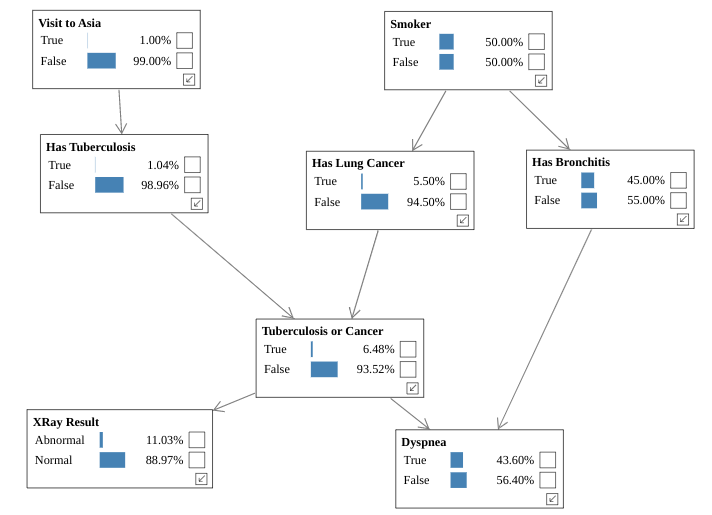
\includegraphics[width=0.7\textwidth]{bayesian-asia-network.png}
	\caption{Example of Bayesian network: the Asia network (\href{https://www.bayesserver.com/examples/networks/asia}{src}).}
	\label{fig:bayesian-asia-network}
\end{figure}

They are useful in a variety of tasks
\begin{itemize}
	\item Descriptive analytic
	\item Diagnostic analytic
	\item Predictive analytic
	\item Prescriptive analytic
\end{itemize}

\backmatter
\pagenumbering{Roman}
\printbibliography[heading=bibintoc]
\appendix
\end{document}